\section{Architectural Overview: Basic TC System}

The \tcs system includes three main components: The \tcontract, the \encname, and the \medname.

The \tcontract (denoted more concisely by \tcont) is a smart contract that acts as the blockchain front-end of the \tc service, and thus an interface between relying contracts and \tc. It accepts datagram requests from requesters and returns corresponding datagrams from \tc. Additionally, the \tcontract manages \tc monetary resources, both fees and gas (in Ethereum). 

The \encname and \medname reside on the \tc server. The \encname runs in an enclave, an SGX-protected execution environment in the server. As enclaves lack network access, the \medname handles bidirectional network traffic on behalf of the \encname, providing network connectivity to the blockchain (the Ethereum system) and to data sources queried by \encname. Additionally, \medname acts as a web server handling off-chain service requests from clients. The \medname is an ordinary user-space application. It does not benefit from special hardware protection and thus, unlike the \encname, can be subverted by an adversarial OS on the \tc server, causing network delays or failures.

The \encname ingests and fulfills datagram requests. To obtain the data composing datagrams, it queries external data sources, specifically HTTPS-enabled internet services. To obtain and keep track of the state of datagram requests, it monitors the state of \tcontract on the blockchain; thus \tcontract forwards datagram requests implicitly to the \tc server. (In the initial version of \tcontract, the \encname's view of the blockchain also comes from a data source.) 

Briefly, then, the end-to-end processing of a datagram request is initiated by a requester \reqcont. \reqcont sends a datagram request to \tcont on the blockchain. Using network services provided by the \medname, the \encname obtains the request from the blockchain. It contacts a data source to obtain the requested data and composes a datagram, which it sends back to \reqcont. Figure~\ref{fig:overview} shows a basic schematic of the \tc system.

As a simple example, \reqcont might request a stock ticker value (e.g., the price of IBM at 3 p.m. on 15 Jan 2016). The \encname would fetch the requested data from an online service (e.g., https://www.google.com/finance) and place it in a datagram for transmission via \tcont to \reqcont.

In addition to servicing datagram requests, the \encname may be queried by a client to provide supplies off-chain, hardware-backed attestations on the state of the \encname---both its executing code and its clock. It is to support this service that \medname includes a web server. We do not depict this service in Figure~\ref{fig:overview}, and defer its discussion to later in the paper.

\vspace{-2mm}
\begin{figure}[h!]
\centering
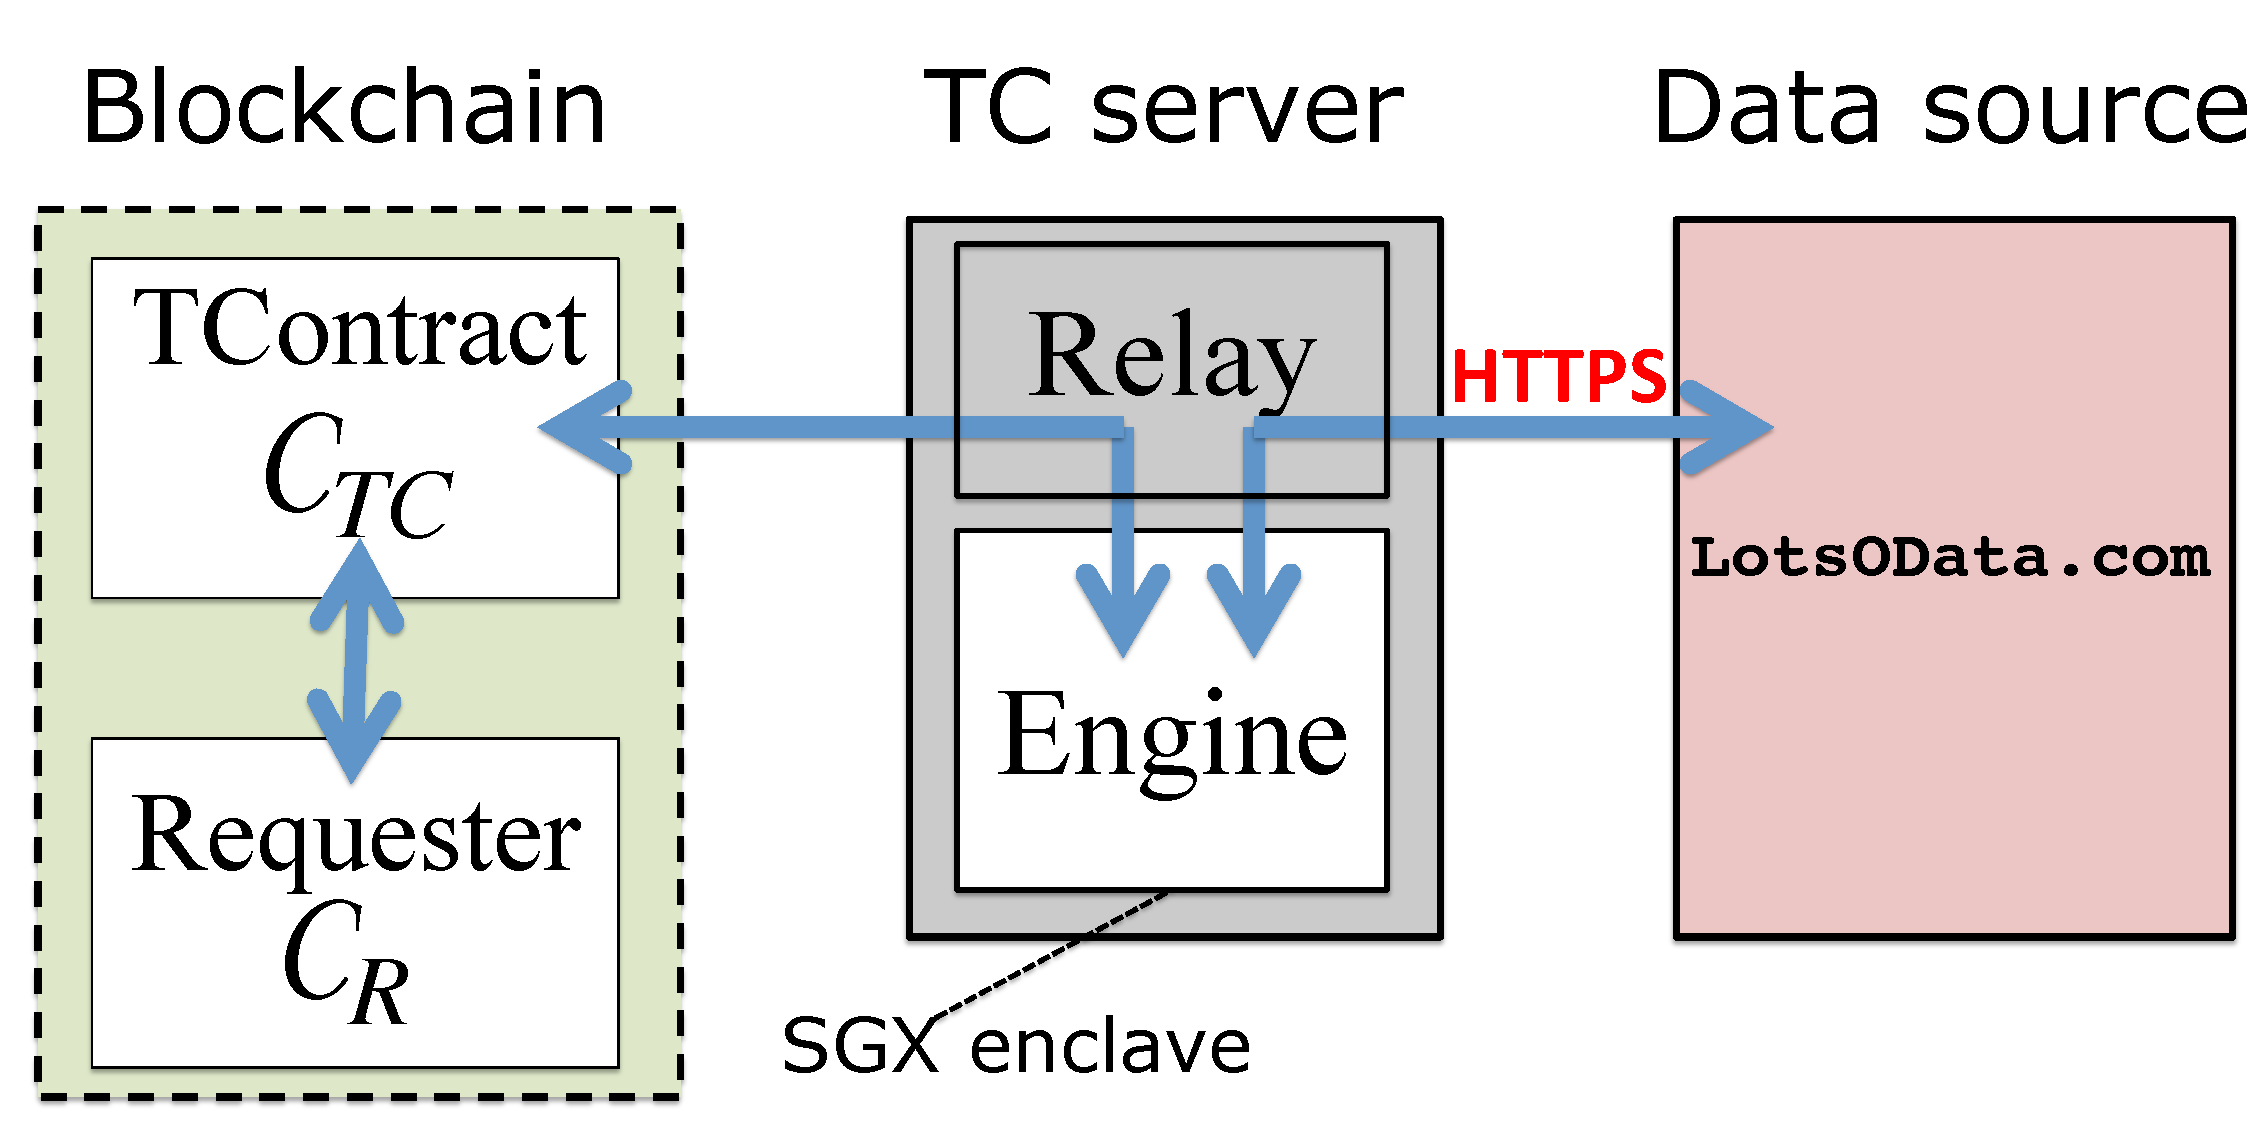
\includegraphics[width=\columnwidth]{OverviewFig}
\caption{{\bf Basic Town Crier architecture.}}
\label{fig:overview}
\end{figure}
\vspace{-2mm}

We now explain in detail the data flow around a datagram request. 

\subsection{Data flow and notation}

We denote a datagram instance, namely the set of message values associated with a datagram request, by $\dg$. Due to the idiosyncracies of Ethereum and the use of digital signatures for message authentication, the full cycle of datagram processing involves a number of messages. 

A datagram request by \reqcont takes the form of a message $\dgreq$ to \tcont on the blockchain. This message $\dgreq$ includes both a specification $\dgform$ of the requested datagram (e.g., a stock ticker and desired time) and a payment $\dgpay$, which includes (in Ethereum) gas to cover the cost of the request as well as a fee. \tcont receives a return message $\dgret$ from the $\tc$ service. In Ethereum, messages are sent from wallet (non-contract) addresses, not contracts. Thus \tc makes use of an address \tcadd on the blockchain to transmit $\dgret$ to \tcont. 
On receiving $\dgret$, \tcont returns the data $\dgm$ it contains (e.g., the desired stock ticker value) to \reqcont. 

We use $\dgi$ to indicate a unique index for a datagram instance. Messages from wallet addresses are authenticated via digital signatures. We use $(\skA, \pkA)$ to denote the private / public key pair associated with \tcadd. The key $\skA$ is stored inside the \encname. 


\subsection{Client API}
\subsection{TC server}
\subsubsection{Trusted executable}
\subsubsection{Untrusted executable}
\subsection{TC Blockchain resources}
These include the TC contract and the addresses from which it sends messages and manages its wallet
\subsection{Security model}


